\documentclass[10pt,letterpaper]{article}
\usepackage[top=1in,bottom=1in,left=1in,right=1in]{geometry}
\usepackage{datetime}
\usepackage{natbib}      % http://merkel.zoneo.net/Latex/natbib.php
\usepackage{palatino}
\usepackage{verbatim}
\usepackage[normalem]{ulem}
\bibpunct{(}{)}{;}{a}{,}{,}

\usepackage{array}

\usepackage{chngpage}
\usepackage{stmaryrd}
\usepackage{amssymb}
\usepackage{amsmath}
\usepackage{graphicx}
\usepackage{lscape}
\usepackage{subfigure}
\usepackage[usenames,dvipsnames]{color}
\definecolor{myblue}{rgb}{0,0.1,0.6}
\definecolor{mygreen}{rgb}{0,0.3,0.1}
\usepackage[colorlinks=true,linkcolor=black,citecolor=mygreen,urlcolor=myblue]{hyperref}

\newcommand{\bocomment}[1]{\textcolor{Bittersweet}{BO says: #1}}
\newcommand{\ignore}[1]{}
\newcommand{\transpose}{^\mathsf{T}}
\newcommand{\inner}[1]{\langle #1 \rangle} 
\newcommand{\smallsec}[1]{\noindent \textbf{#1\ }}
\newcommand{\cmd}[1] {{\color{blue}\texttt{#1}}}

\newcommand{\solution}[1]{{\color{myblue} \emph{[Solution:} 

#1 

\emph{End solution]}}}
\newcommand{\solutionnote}[1]{{\color{myblue} \emph{[Note:}

#1 

\emph{End note]}}}
\newcommand{\points}[1]{{\color{mygreen}\emph{[#1]\ \ }}}

\newcommand{\aone}{\diamondsuit}
\newcommand{\atwo}{\heartsuit}
\newcommand{\bone}{\triangle}
\newcommand{\btwo}{\Box}
\newcommand{\myand}{\ \land\ }
\newcommand{\myor}{\ \lor\ }
\newcommand{\mynot}{\lnot}

\title{
  Mini-project 3\\
  \Large{COMPSCI 370, Spring 2021, UMass Amherst} \\
  \Large{Instructor: Subhransu Maji} \\
  \Large{TAs: Chenyun Wu, Jong-Chyi Su}
}

\settimeformat{ampmtime}
\date{}
\begin{document}
\maketitle

\renewcommand\thesubsection{\thesection.\alph{subsection}}
\section*{Guidelines}
\paragraph{Submission.} Submit a \emph{single pdf} file via
Gradescope that includes your solutions, figures, and code. The latex
source file for the homework is provided in case you want to modify it
to produce your report. However, you are welcome to use other
typesetting software as long as the final output is a pdf.
For readability you may attach the code printouts at the end of the
solutions within the same pdf.
Similarly figures enable easy comparision of various approaches.
Poorly written or formatted reports will make it harder for us to
evaluate it and may lead to a deduction of credit.


\paragraph{Late policy.}
\begin{itemize}
\item You can use 7 late days, with up to 3 late days per assignment.
\item Once you have used all 7 late days, penalty is 25\% for each additional late day.
\item We will use your latest submission for grading and for calculating your late day usage.
\item There is no bonus if you don't use late days at all.
\end{itemize}


\paragraph{Plagiarism.}
We expect the students not to copy, refer to, or look at the solutions
in preparing their answers. We expect students to want to learn and
not google for answers. See the Universities' guidelines on academic
honesty (\url{https://www.umass.edu/honesty}).
Finally, we also ask you to not post the solutions online as the
problem sets might be used in future.


\paragraph{Collaboration.} The homework must be done individually,
except where otherwise noted in the assignments. 'Individually' means
each student must hand in their own answers, and each student must
write their own code in the programming part of the assignment. It is
acceptable, however, for students to collaborate in figuring out
answers and helping each other solve the problems, for example within
a study group.
We will be assuming that you will be taking the responsibility to make
sure you personally understand the solution to any work arising from
such a collaboration.


\paragraph{Python requirements.}
Our code is tested on Python 3.
The Python code depends on external
packages such as \cmd{scipy}, \cmd{numpy}, and \cmd{scikit-image}.
Take a look at the resources posted on the course page to set up the
appropriate programming environment and tutorial on basic concepts.


\paragraph{Using other programming languages.}
While we have made the starter code available in Python, 
feel free to implement the homework from scratch using your favorite
programming language. For example you are welcome to use Matlab, C, Java,
Octave or Julia, with the caveat that we may be able help you with
debugging.







\newpage


%%%%%%%%%%%%%%%%%%%%%%%%%%%%%%%%%%%%
\section{Improving image constrast [20 points]}
You will implement \emph{contrast stretching}, \emph{gamma correction},
and \emph{histogram equalization} for enhancing the contrast.
All these techniques are based on remapping brightness values of
pixels in an image.

\begin{figure}[h]
\begin{tabular}{cc}
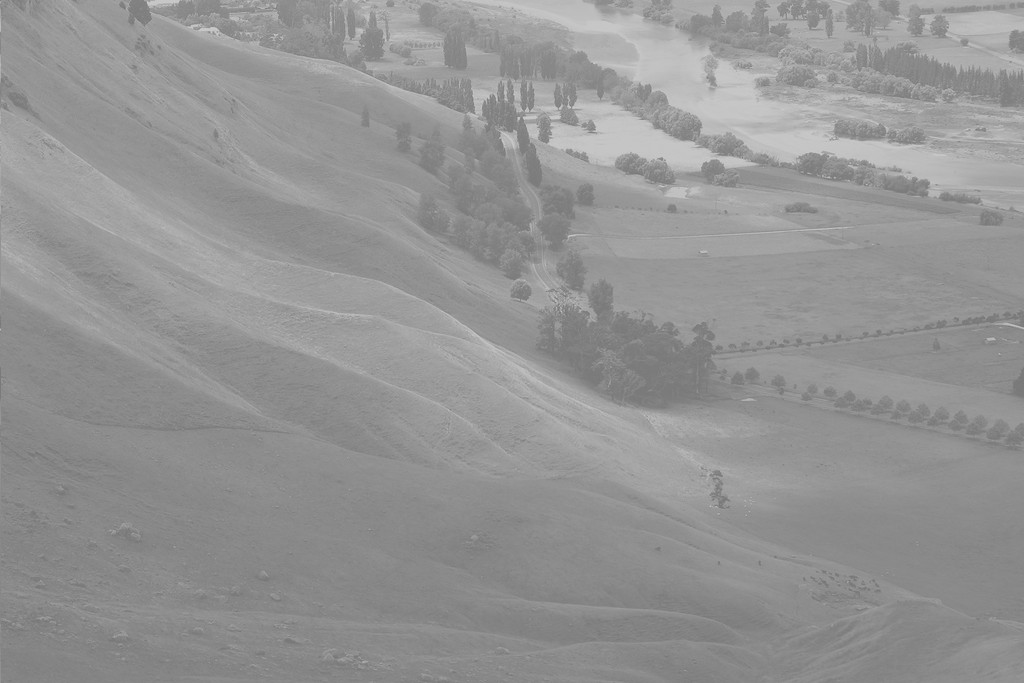
\includegraphics[width=0.33\linewidth,height=0.18\textheight]{fig/hills.jpg}
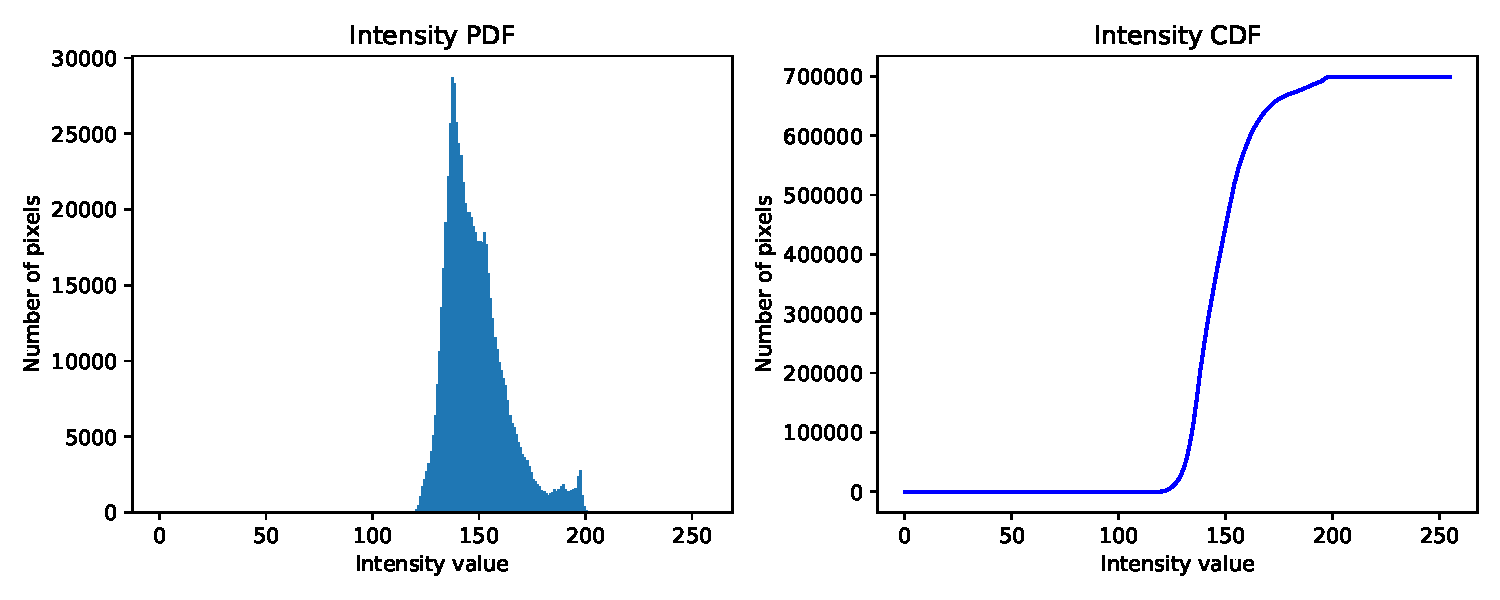
\includegraphics[width=0.66\linewidth,height=0.18\textheight]{fig/hills-hist.pdf} \\
%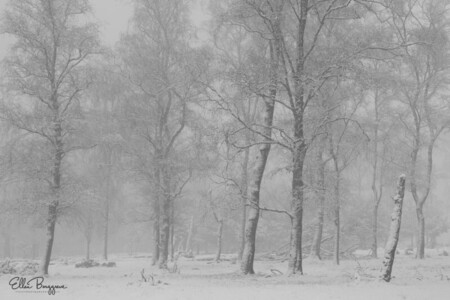
\includegraphics[width=0.33\linewidth,height=0.18\textheight]{fig/forest.png}
%\includegraphics[width=0.66\linewidth,height=0.18\textheight]{fig/forest-hist.pdf} \\
\end{tabular}
\caption{\label{fig:original} An example of an image and its pdf and cdf.}
\end{figure}



\begin{itemize}

\item \points{5 points} Implement a function \cmd{[pdf,cdf] =
  histogram(im)} that computes the \emph{probability density function}
  (pdf) and
  \emph{cumulative distribution function} (cdf) for an image
  \cmd{im}. Assume that \cmd{im} is a grayscale image with
  brightness values $\in [0,255]$. The pdf is array of size 256
  where
  $$
  \text{pdf[i] = number of pixels in im with value $=$ i, for i } \in \{0,1,\ldots, 255\}.
  $$
  Similarly the cdf is an array where 
  $$
  \text{cdf[i] = number of pixels in im with value $\leq$ i, for i } \in
  \{0, 1, \ldots, 255\}.
  $$
  Note that your implementation should loop over pixels and compute
  these quantities and {\color{red}not use inbuilt functions to compute the histogram such as \cmd{np.histogram} or \cmd{np.bincount}}. 
  The cdf and pdf should be represented as numpy ndarrays.
  Also note that the cdf
  can be computed from the pdf directly.
  Visualize the pdf and cdf on the image \cmd{forest.png} provided
  in the \cmd{data} folder in the format shown
  above, where the pdf is shown as a histogram and the cdf is plotted
  as a line. You can use \cmd{pyplot.bar} to plot a histogram and
  \cmd{pyplot.plot} to plot the cdf with \cmd{matplotlib}.
  {\color{red}{Note: please use \cmd{forest.png} as the input for all the following questions.}}
 
\item \points{5 points} Implement contrast stretching which maps the
  minimum pixel value to 0 and the maximum pixel value to 255. The
  pixel values in between are linearly interpolated.
  Specifically, a pixel value $v$ mapped to
\[
h(v) =  \texttt{round} \left(  \frac{v-\min(im)}{\max(im) - \min(im)} \times 255 \right). 
\]
Apply this mapping to the provided image.
Show the image after the transformation and plot the pdf (histogram) and cdf of the image as in Figure~\ref{fig:original}.

\item \points{5 points} Gamma correction uses the following mapping function for pixel values:
\[
h(v) = \texttt{round}\left(  \left(\frac{v}{255}\right)^{\gamma} \times 255 \right).
\]
Implement this function and generate images with $\gamma = 2$ and $\gamma = 0.5$. 
Show the images and plot their resulting pdf and cdf for both values of $\gamma$.
What is the qualitative effect of $\gamma$ on these images? 

\item \points{5 points} Histogram equalization remaps the values to
  achieve a uniform distribution of the cdf. In class we showed that
  the mapping that achieves this is:
\[
h(v) = \texttt{round}\left(  \frac{cdf(v) - cdf_{\min}}{N - cdf_{\min}} \times 255 \right),
\]
where N is the number of the pixels in the image, and $cdf_{min}$ is the number (of the pixels) in the first non-zero bin of the cdf.
Implement this function and apply it on the image. 
Once again, show the image after the transformation and visualize the pdf and cdf. 
\end{itemize}


%%%%%%%%%%%%%%%%%%%%%%%%%%%%%%%%%%%%
\section{Image denoising [15 points]}
In this part you will evaluate Gaussian filtering and median filtering
for image denoising. You are provided with
\begin{itemize}
\item \texttt{peppers.png} -- reference image without noise
\item \texttt{peppers\_g.png}  -- image with Gaussian noise. 
\item \texttt{peppers\_sp.png}  -- image with ``Salt and Pepper" noise.
\end{itemize}

%The two versions correspond to different amounts of noise.
The \cmd{evalDenoising.py} script loads three images, visualizes them, and
computes the error (squared-distance) between them as shown
below.
Your goal is to denoise the images which should result in a
lower error value.


\begin{figure}[h]
\centering
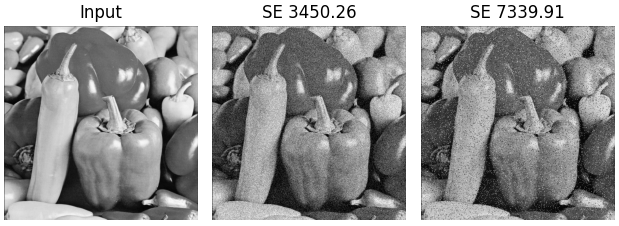
\includegraphics[width=0.8\linewidth]{fig/denoising-output-peppers.png}
\caption{\label{fig:bayer} Input images for denoising and their errors (squared-distance).}
\end{figure}

\begin{itemize}
\item \points{5 points} Using \cmd{scipy.ndimage.gaussian\_filter}
  apply Gaussian filter on the above images.
  Experiment with different values of the
  standard deviation parameter $\sigma$. Report the optimal error and
  $\sigma$ for each of these images.
 
\item \points{5 points} Using \cmd{scipy.ndimage.median\_filter} apply
  a median filter on the above images. Report the optimal error and neighborhood
  size for each of the images.
  
\item \points{5 points} Qualitatively compare the outputs of these
  results. You should include the outputs of the algorithms
  side-by-side for an easy comparison. Which algorithm works the best
  for which image?

\end{itemize}


%%%%%%%%%%%%%%%%%%%%%%%%%%%%%%%%%%%%
\section{Hybrid images [20 points]}
A hybrid image is a sum of blurry image and a sharpened image that looks like one or
the other depending on the perceived resolution of the image. In this part you will try to create such images.
Recall that one can obtain a sharp image by subtracting the blurry
version of an image from itself. Mathematically we have

\[
	I = \texttt{blurry}(I) + \texttt{sharp}(I).
\]

A blurry image can be obtained by filtering an image with
a Gaussian. Thus, a hybrid image of $I_1$ and $I_2$ can be obtained by
\begin{equation}\label{eq:hybrid}
	I_{hybrid} = \texttt{blurry}(I_1, \sigma_1) + \texttt{sharp}(I_2, \sigma_2) = I_1 * g(\sigma_1) + I_2 - I_2*g(\sigma_2)
\end{equation}

where, $g(\sigma_1)$ and $g(\sigma_2)$ are Gaussian filters with
parameters $\sigma_1$ and $\sigma_2$ and * denotes the filtering
operator.
Figure~\ref{fig:blur} shows the result of convolution with Gaussian filters with two different values of $\sigma$. 



\begin{figure}[h]
\begin{tabular}{cccc}
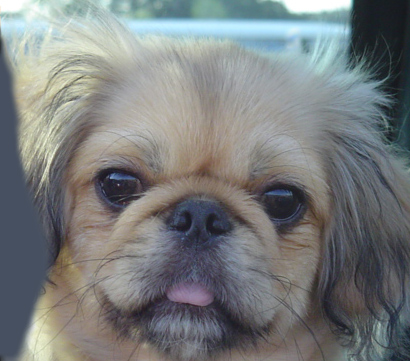
\includegraphics[width=0.23\linewidth]{fig/dog.jpg} &
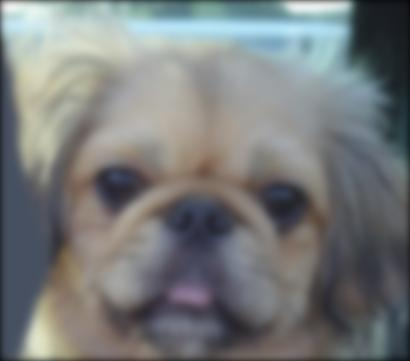
\includegraphics[width=0.23\linewidth]{fig/dog-blurry-4.jpg} & 
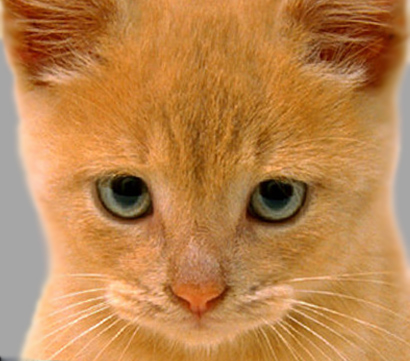
\includegraphics[width=0.23\linewidth]{fig/cat.jpg} &
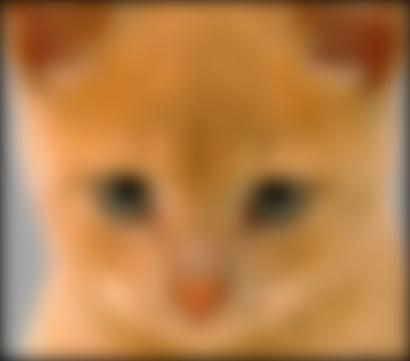
\includegraphics[width=0.23\linewidth]{fig/cat-blurry-10.jpg}\\
dog image & $\sigma=4$ & cat image & $\sigma=10$ \\
\end{tabular}
\caption{\label{fig:blur} Effect of filtering with a Gaussian. The bigger the sigma the more blurry it is.}
\end{figure}

\begin{itemize}

\item \points{20 points} Implement the function 
$\cmd{hybridImage(im1, im2, sigma1, sigma2)}$ that computes the hybrid
  image using Equation~\ref{eq:hybrid}. Use your code to generate at
  least one example of a hybrid image (see examples here
  \url{http://cvcl.mit.edu/hybrid_gallery/gallery.html}). You will
  have to tune the $\cmd{sigma1}$ and $\cmd{sigma2}$ to make it work
  on specific images. In order to visualize the hybrid image it is
  useful to show multiple copies of the image at different
  resolutions.
The codebase includes a helper function $\cmd{vis\_hybrid\_image}$ which can be used to create such a figure.
In Python, \cmd{matplotlib} does not handle negative values in images,
so use \cmd{np.clip} to make sure that image values are
between 0 and 1 (assuming floating point representation).
Include the code, the two source images, the hybrid image displayed in
the format below, as well as the parameters that worked for you. The
top three submissions (judged based on creativity and how compelling it is) will be announced in class.

\end{itemize}
\begin{figure}[h]
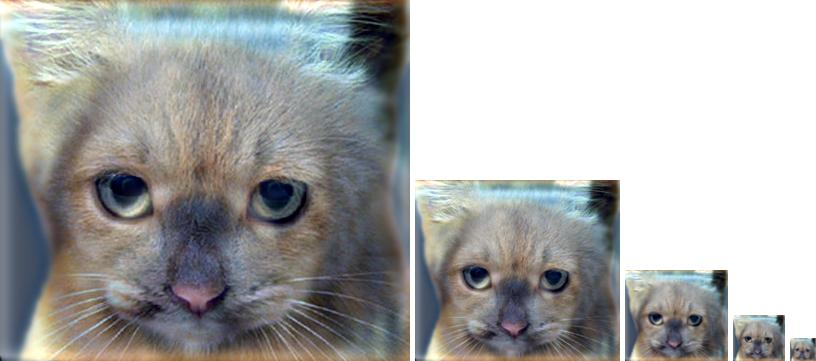
\includegraphics[width=\linewidth]{fig/hybrid-4-10.jpg}
\caption{Hybid image of the dog and cat. The large image looks like
  the cat while the small image looks like the dog. The image was
  created with $\sigma_1 = 4$ and $\sigma_2 = 10$.}
\end{figure}


\end{document}
